%% eval.tex
%% $Id: eval.tex 5 2005-10-10 20:55:48Z bless $

\chapter{Evaluation}
\label{ch:Evaluation}
Die Evaluation der Ergebnisse beginnt damit, die Daten der eSense Earpods in Fenster (\textit{windows}) einzuteilen.
Auf diese Fenster werden anschließend \textit{Features} berechnet, welche die Grundlage für die Klassifizierung sind.

\section{Gibt es passende Features?}
Die Suche nach passenden Features wird mit dem Python Package \texttt{tsfresh} angegangen.
\texttt{tsfresh} berechnet automatisch Charakteristiken, sowie deren Relevanz anhand eines Zeitintervalls (\textit{Feature}) \todo{ref to website https://tsfresh.readthedocs.io}.
Diese Charakteristiken werden fortan als Features bezeichnet. \todo{wo steckt die relevanz in den tsfresh daten... }

Als Eingabe bekommt \texttt{tsfresh} die Daten der eSense Earpods, also die \textit{x, y} und \textit{z}- Achse der Gyroskop und Beschleunigungsdaten, versehen mit einem Zeitstempel. 
Anhand dieser Informationen berechnet \texttt{tsfresh} nun ($\sim$ 6000) Features für jedes Fenster.

\section{Ablauf der Evaluierung}
Im Kapitel \ref{ch:Implementierung:classification_pipeline} wurde beschrieben, wie die Features berechnet und persistiert wurden. 
Nun sind pro Studienteilnehmer für alle 3 Positionen Features berechnet worden. 
Es sind jeweils die Features für ein Fenster von 5 Sekunden und 10 Sekunden berechnet worden.
Zur Erinnerung: Jede Messung wurde in Fenster der Länge von 5, bzw. 10 Sekunden aufgeteilt, wobei jedes Fenster um eine Sekunde verschoben ist.

\subsection{Data Labeling}
Zur Klassifikation müssen die Daten bereits markiert sein, um eine Entscheidung treffen zu können. 
Beim Abspeichern der eSense Daten ist dies bereits geschehen. 
Da die Messung genau vorgibt, wann eine Person die luft anhalten soll, beziehungsweise nicht, wird diese Information mit einem \textit{Boolean} als zusätzliches Attribut vermerkt.
Da bei der Klassifikation Features anhand der eSense Daten berechnet werden, darf dieses Attribut offensichtlich nicht Teil der Featureberechnung sein.
Da nun bei einem 5 Sekunden Intervall circa 250 Einträge, bei einem 10 Sekunden Intervall circa 500 Einträge in eine Featureberechnung zusammenfließen, muss die Markierung dieses Features berechnet werden.
Ab 50\% der markierten Einträge wird das ganze Intervall als markiert gesetzt.
Dies ist eine essenzielle Entscheidung, da beim Training des Modells nun anhand dieser Markierung entschieden wird, ob ein Intervall ein Atemaussetzer repräsentiert, oder nicht.
\todo{genauer beschreiben, warum hier 50\% gewählt wurde... ich wollte bei 90\% z.B die Übergänge nicht als 0 markieren, weil dann teile der 0 markierten features eigentlich ein Atemaussetzer gewesen wäre... dann trainiert es kacke...}
Nun können die Resultate mit den Klassifikatoren verglichen werden.

\subsection{Methoden}
\subsubsection{Kreuzvalidierungsverfahren}
Die Klassifikation wurde mit verschiedenen Verfahren durchgeführt. 
Die erste Methode ist das Kreuzvalidierungsverfahren. 
Hierbei wird ein Modell anhand der Daten der Studienteilnehmer trainiert, jedoch wird ein Datensatz eines Studienteilnehmers ausgelassen. 
Dieser eine Datensatz wird schließlich verwendet, um eine Vorhersage anhand der Trainingsdaten zu treffen, ohne durch interne Trainingsdaten optimiert sein zu können.
Im Folgenden wurde das Kreuzvalidierungsverfahren durchgeführt mit den beiden Klassifikationsalgorithmen \textit{Random Forest} und \textit{XGBoost}. 
Es wurde jede Person einmal ausgelassen und auf den Trainingsdatensatz angewandt, welcher diese Person nicht enthält. 
Somit entstehen 7 Resultate, von denen nun der Mittelwert gebildet wird.
Die Resultate sind in den Abbildungen \ref{evaluation:random_forest_loso_5:person6}, \ref{evaluation:random_forest_loso_10:person6}, \ref{evaluation:xgboost_loso_5:person6}, \ref{evaluation:xgboost_loso_10:person6} dargestellt.
Die vollständige Auflistung aller Resultate sind im Anhang zu finden. \\
Hier ist anzumerken, dass Person 6 als Beispiel genommen wurde. 
Es wurde eine Vorhersage auf jede Person einzeln getroffen, welche dann im \textit{Precision} und \textit{Recall} der unterliegenden Tabelle mit dem Mittelwert zusammengetragen wurden. 

Des weiteren, um mögliche Positionsabhängigkeiten zu erkennen, wurden das selbe erneut evaluiert, jedoch nur mit den einzelnen Positionsdaten der jeweiligen Person. 
In Abbildung \ref{asdf} \todo{add ref} sind die Resultate zu sehen.

%%%%%%%%%%%%%%%%%%%        RANDOM FOREST 5 sec %%%%%%%%%%%%%%%%%%%%%%%%%%%%%%%%%
\begin{figure}[ht]
    \centering
    \begin{subfigure}{1\textwidth}
        \includegraphics[width=1\textwidth]{evaluation/loso_5sec/random_forest_loso/Random Forest (Leave one Subject out: Person 6 back).png}
        \caption{Klassifikationsresultate der Person 6. Die Messung wurde auf dem Rücken liegend durchgeführt.}
      \end{subfigure}
      \begin{subfigure}{1\textwidth}
        \includegraphics[width=1\textwidth]{evaluation/loso_5sec/random_forest_loso/Random Forest (Leave one Subject out: Person 6 side).png}
        \caption{Klassifikationsresultate der Person 6. Die Messung wurde auf der Seite liegend durchgeführt.}
      \end{subfigure}
      \begin{subfigure}{1\textwidth}
        \includegraphics[width=1\textwidth]{evaluation/loso_5sec/random_forest_loso/Random Forest (Leave one Subject out: Person 6 stomach).png}
        \caption{Klassifikationsresultate der Person 6. Die Messung wurde auf dem Bauch liegend durchgeführt.}
    \end{subfigure}
    \label{evaluation:random_forest_loso_5:person6}

    \begin{subfigure}{1\textwidth}
        \begin{center}
            \begin{tabular}{ | l | c | r | }
              \hline
               & precision & recall \\ \hline
              0 & 0.92054 & 0.74887 \\ \hline
              1 & 0.74887 & 0.66565 \\
              \hline
            \end{tabular}
        \end{center}
        \caption{Random Forest mit dem Kreuzvalidierungsverfahren}
        \label{implementation:app:screenshots:user_studies_information}
    \end{subfigure}
    \caption{Ergebnisse eines Kreuzvalidierungsverfahren der Person 6 mit dem Klassifikationsalgorithmus Random Forest und einer Fenstergröße von 5 Sekunden mit einer Verschiebung der Fenster von 1 Sekunde. Hier wurden alle Positionen mit in das Modell zum trainieren gegeben und es wurde auf alle Positionen der Person 6 vorhergesagt. Die blauen Bereiche sind die, in denen die Luft angehalten wurde, die orangene Kurve ist die Vorhersage.}
\end{figure}

%%%%%%%%%%%%%%%%%%%        RANDOM FOREST 10 sec %%%%%%%%%%%%%%%%%%%%%%%%%%%%%%%%%
\begin{figure}[ht]
    \centering
    \begin{subfigure}{1\textwidth}
        \includegraphics[width=1\textwidth]{evaluation/loso_10sec/random_forest_loso/Random Forest (Leave one Subject out: Person 6 back).png}
        \caption{Klassifikationsresultate der Person 6. Die Messung wurde auf dem Rücken liegend durchgeführt.}
      \end{subfigure}
      \begin{subfigure}{1\textwidth}
        \includegraphics[width=1\textwidth]{evaluation/loso_10sec/random_forest_loso/Random Forest (Leave one Subject out: Person 6 side).png}
        \caption{Klassifikationsresultate der Person 6. Die Messung wurde auf der Seite liegend durchgeführt.}
      \end{subfigure}
      \begin{subfigure}{1\textwidth}
        \includegraphics[width=1\textwidth]{evaluation/loso_10sec/random_forest_loso/Random Forest (Leave one Subject out: Person 6 stomach).png}
        \caption{Klassifikationsresultate der Person 6. Die Messung wurde auf dem Bauch liegend durchgeführt.}
    \end{subfigure}
    \label{evaluation:random_forest_loso_10:person6}

    \begin{subfigure}{1\textwidth}
        \begin{center}
            \begin{tabular}{ | l | c | r | }
              \hline
               & precision & recall \\ \hline
              0 & 0.91499 & 0.76483 \\ \hline
              1 & 0.76483 & 0.67411 \\
              \hline
            \end{tabular}
        \end{center}
        \caption{Random Forest mit dem Kreuzvalidierungsverfahren}
        \label{implementation:app:screenshots:user_studies_information}
    \end{subfigure}
    \caption{Ergebnisse eines Kreuzvalidierungsverfahren der Person 6 mit dem Klassifikationsalgorithmus Random Forest und einer Fenstergröße von 10 Sekunden mit einer Verschiebung der Fenster von 1 Sekunde. Hier wurden alle Positionen mit in das Modell zum trainieren gegeben und es wurde auf alle Positionen der Person 6 vorhergesagt. Die blauen Bereiche sind die, in denen die Luft angehalten wurde, die orangene Kurve ist die Vorhersage.}
\end{figure}

%%%%%%%%%%%%%%%%%%%        XG BOOST 5 sec %%%%%%%%%%%%%%%%%%%%%%%%%%%%%%%%%

\begin{figure}[ht]
    \centering
    \begin{subfigure}{1\textwidth}
        \includegraphics[width=1\textwidth]{evaluation/loso_5sec/xg_boost_loso/XG Boost (Leave one Subject out: Person 6 back).png}
        \caption{Klassifikationsresultate der Person 6. Die Messung wurde auf dem Rücken liegend durchgeführt.}
      \end{subfigure}
      \begin{subfigure}{1\textwidth}
        \includegraphics[width=1\textwidth]{evaluation/loso_5sec/xg_boost_loso/XG Boost (Leave one Subject out: Person 6 side).png}
        \caption{Klassifikationsresultate der Person 6. Die Messung wurde auf der Seite liegend durchgeführt.}
      \end{subfigure}
      \begin{subfigure}{1\textwidth}
        \includegraphics[width=1\textwidth]{evaluation/loso_5sec/xg_boost_loso/XG Boost (Leave one Subject out: Person 6 stomach).png}
        \caption{Klassifikationsresultate der Person 6. Die Messung wurde auf dem Bauch liegend durchgeführt.}
    \end{subfigure}
    \label{evaluation:xgboost_loso_5:person6}

    \begin{subfigure}{1\textwidth}
        \begin{center}
            \begin{tabular}{ | l | c | r | }
              \hline
               & precision & recall \\ \hline
              0 & 0.93269 & 0.69694 \\ \hline
              1 & 0.69694 & 0.72791 \\
              \hline
            \end{tabular}
        \end{center}
        \caption{XGBoost mit dem Kreuzvalidierungsverfahren}
        \label{implementation:app:screenshots:user_studies_information}
    \end{subfigure}
    \caption{Ergebnisse eines Kreuzvalidierungsverfahren der Person 6 mit dem Klassifikationsalgorithmus XGBoost und einer Fenstergröße von 5 Sekunden mit einer Verschiebung der Fenster von 1 Sekunde. Hier wurden alle Positionen mit in das Modell zum trainieren gegeben und es wurde auf alle Positionen der Person 6 vorhergesagt. Die blauen Bereiche sind die, in denen die Luft angehalten wurde, die orangene Kurve ist die Vorhersage.}
\end{figure}

%%%%%%%%%%%%%%%%%%%        XG BOOST 10 sec %%%%%%%%%%%%%%%%%%%%%%%%%%%%%%%%%
\begin{figure}[ht]
    \centering
    \begin{subfigure}{1\textwidth}
        \includegraphics[width=1\textwidth]{evaluation/loso_10sec/xg_boost_loso/XG Boost (Leave one Subject out: Person 6 back).png}
        \caption{Klassifikationsresultate der Person 6. Die Messung wurde auf dem Rücken liegend durchgeführt.}
      \end{subfigure}
      \begin{subfigure}{1\textwidth}
        \includegraphics[width=1\textwidth]{evaluation/loso_10sec/xg_boost_loso/XG Boost (Leave one Subject out: Person 6 side).png}
        \caption{Klassifikationsresultate der Person 6. Die Messung wurde auf der Seite liegend durchgeführt.}
      \end{subfigure}
      \begin{subfigure}{1\textwidth}
        \includegraphics[width=1\textwidth]{evaluation/loso_10sec/xg_boost_loso/XG Boost (Leave one Subject out: Person 6 stomach).png}
        \caption{Klassifikationsresultate der Person 6. Die Messung wurde auf dem Bauch liegend durchgeführt.}
    \end{subfigure}
    \label{evaluation:xgboost_loso_10:person6}

    \begin{subfigure}{1\textwidth}
        \begin{center}
            \begin{tabular}{ | l | c | r | }
              \hline
               & precision & recall \\ \hline
              0 & 0.93186 & 0.74072 \\ \hline
              1 & 0.74072 & 0.74767 \\
              \hline
            \end{tabular}
        \end{center}
        \caption{XGBoost mit dem Kreuzvalidierungsverfahren}
        \label{implementation:app:screenshots:user_studies_information}
    \end{subfigure}
    \caption{Ergebnisse eines Kreuzvalidierungsverfahren der Person 6 mit dem Klassifikationsalgorithmus XGBoost und einer Fenstergröße von 10 Sekunden mit einer Verschiebung der Fenster von 1 Sekunde. Hier wurden alle Positionen mit in das Modell zum trainieren gegeben und es wurde auf alle Positionen der Person 6 vorhergesagt. Die blauen Bereiche sind die, in denen die Luft angehalten wurde, die orangene Kurve ist die Vorhersage.}
\end{figure}

%%%%%%%%%%%%%%%%%%%        Position based results  5 sec %%%%%%%%%%%%%%%%%%%%%%%%%%%%%%%%%
\todo{add description for each table}


\begin{tabular}{cc}    
    \begin{minipage}{.33\linewidth}
        \begin{center}
            \begin{tabular}{ | l | c | r | }
              \hline
               & precision & recall \\ \hline
              0 & 0.89921 & 0.71875 \\ \hline
              1 & 0.71875 & 0.57238 \\
              \hline
            \end{tabular}
        \end{center}
        %\caption{random forest loso side}
        %\label{evaluation:5s:random_forest_loso_side}
    \end{minipage}

    \begin{minipage}{.33\linewidth}
        \begin{center}
            \begin{tabular}{ | l | c | r | }
              \hline
               & precision & recall \\ \hline
              0 & 0.89094 & 0.82538 \\ \hline
              1 & 0.82538 & 0.44796 \\
              \hline
            \end{tabular}
        \end{center}
        %\caption{random forest loso back}
        %\label{evaluation:5s:random_forest_loso_back}
    \end{minipage}

    \begin{minipage}{0.33\textwidth}
        \begin{center}
            \begin{tabular}{ | l | c | r | }
              \hline
               & precision & recall \\ \hline
              0 & 0.92421 & 0.72336 \\ \hline
              1 & 0.723369 & 0.65753 \\
              \hline
            \end{tabular}
        \end{center}
        %\caption{random forest loso stomach}
        %\label{evaluation:5s:random_forest_loso_stomach}
    \end{minipage}
\end{tabular}

\begin{tabular}{cc} 
    \begin{minipage}{0.33\textwidth}
        \begin{center}
            \begin{tabular}{ | l | c | r | }
              \hline
               & precision & recall \\ \hline
              0 & 0.91483 & 0.6697 \\ \hline
              1 & 0.66979 & 0.6116 \\
              \hline
            \end{tabular}
        \end{center}
        %\caption{xg boost loso side}
        %\label{evaluation:5s:xg_boost_loso_side}
    \end{minipage}

    \begin{minipage}{0.33\textwidth}
        \begin{center}
            \begin{tabular}{ | l | c | r | }
              \hline
               & precision & recall \\ \hline
              0 & 0.89937 & 0.75145 \\ \hline
              1 & 0.75145 & 0.54108 \\
              \hline
            \end{tabular}
        \end{center}
        %\caption{xg boost loso back}
        %\label{evaluation:5s:xg_boost_loso_back}
    \end{minipage}

    \begin{minipage}{0.33\textwidth}
        \begin{center}
            \begin{tabular}{ | l | c | r | }
              \hline
               & precision & recall \\ \hline
              0 & 0.94418 & 0.70734 \\ \hline
              1 & 0.70734 & 0.71763 \\
              \hline
            \end{tabular}
        \end{center}
        %\caption{xg boost loso stomach}
        %\label{evaluation:5s:xg_boost_loso_stomach}
    \end{minipage}
\end{tabular}


%%%%%%%%%%%%%%%%%%%        Position based results  10 sec %%%%%%%%%%%%%%%%%%%%%%%%%%%%%%%%%
% \begin{figure}[ht]
%     random_forest_loso_side
% 0 precision: 0.8910321701260353 recall: 0.7944339547679462
% 1 precision: 0.7944339547679462 recall: 0.5342972945135886
% 
% random_forest_loso_back
% 0 precision: 0.8856848120232153 recall: 0.7942768843164358
% 1 precision: 0.7942768843164358 recall: 0.5226600199639415
% 
% random_forest_loso_stomach
% 0 precision: 0.9441160862106648 recall: 0.714477770976837
% 1 precision: 0.714477770976837 recall: 0.7303793266951162
% 
% xg_boost_loso_side
% 0 precision: 0.9049749539351956 recall: 0.7844056251056845
% 1 precision: 0.7844056251056845 recall: 0.6074581770976869
% 
% xg_boost_loso_back
% 0 precision: 0.9030026977390445 recall: 0.7505666120433064
% 1 precision: 0.7505666120433064 recall: 0.5797357581671306
% 
% xg_boost_loso_stomach
% 0 precision: 0.937830526588158 recall: 0.7127870082777301
% 1 precision: 0.7127870082777301 recall: 0.720753883969457
% \end{figure}


Jede Klassifikation ergab ein Resultat, welches durch einzelne Features entschieden wurde. 
Um einen kleinen Überblick zu bekommen, welche Features entscheidend für die Evaluation waren, sind nun einige aufgelistet.
\begin{itemize}
    \item gyroZ partial autocorrelation
    \item gytoX fft coefficient
    \item gyroX agg autocorrelation
    \item accY autocorrelation
    \item gyroY change quantiles 
    \item gyroZ fft coefficient
\end{itemize}
Diese Features wurden mittels \texttt{tsfresh} berechnet und waren bei der Klassifikation des Kreuzvalidierungsverfahrens entscheidened.

\subsubsection{Leave one subject in}
s

Was bieten die verfahren, wie macht das sinn, dass sinnvolle ergebnisse herauskommen...

WelcheVor-undNachteilekönnendieseVerfahrenbieten?

\section{Erkenntnisse}
\todo{ich habe gelernt}
\begin{itemize}
    \item auswertungsdaten: Auf dem rücken liegende ddaten sind am vielversprechendsten
    \item die atempausen können einigermaßen klassifiziert werden
    \item rauschen entfernen bringt nix vermutlich wegen tsfresh, da es das schon macht, also es kommen
    \item 
\end{itemize}


gibt earables, die blutsauerstoff und puls mittracken können
plus grafik telegram tobi